\documentclass[final]{cvpr}

\usepackage{times}
\usepackage{epsfig}
\usepackage{graphicx}
\usepackage{amsmath}
\usepackage{amssymb}
\usepackage{float}
\usepackage{caption}
\usepackage{tikz}
\usetikzlibrary{positioning,arrows.meta,shapes.geometric}
\usepackage[pagebackref=true,breaklinks=true,colorlinks,bookmarks=false]{hyperref}

\begin{document}

%%%%%%%%% TITLE
\title{MedBridge: A Policy-Grounded, Human-in-the-Loop LLM Agent and Chatbot for Healthcare Prior Authorization}

\author{Neha Kumari\\
Northeastern University\\
kumari.neh@northeastern.edu}

\twocolumn[{
    \renewcommand\twocolumn[1][]{#1}%
    \maketitle
    \begin{center}
      \centering
      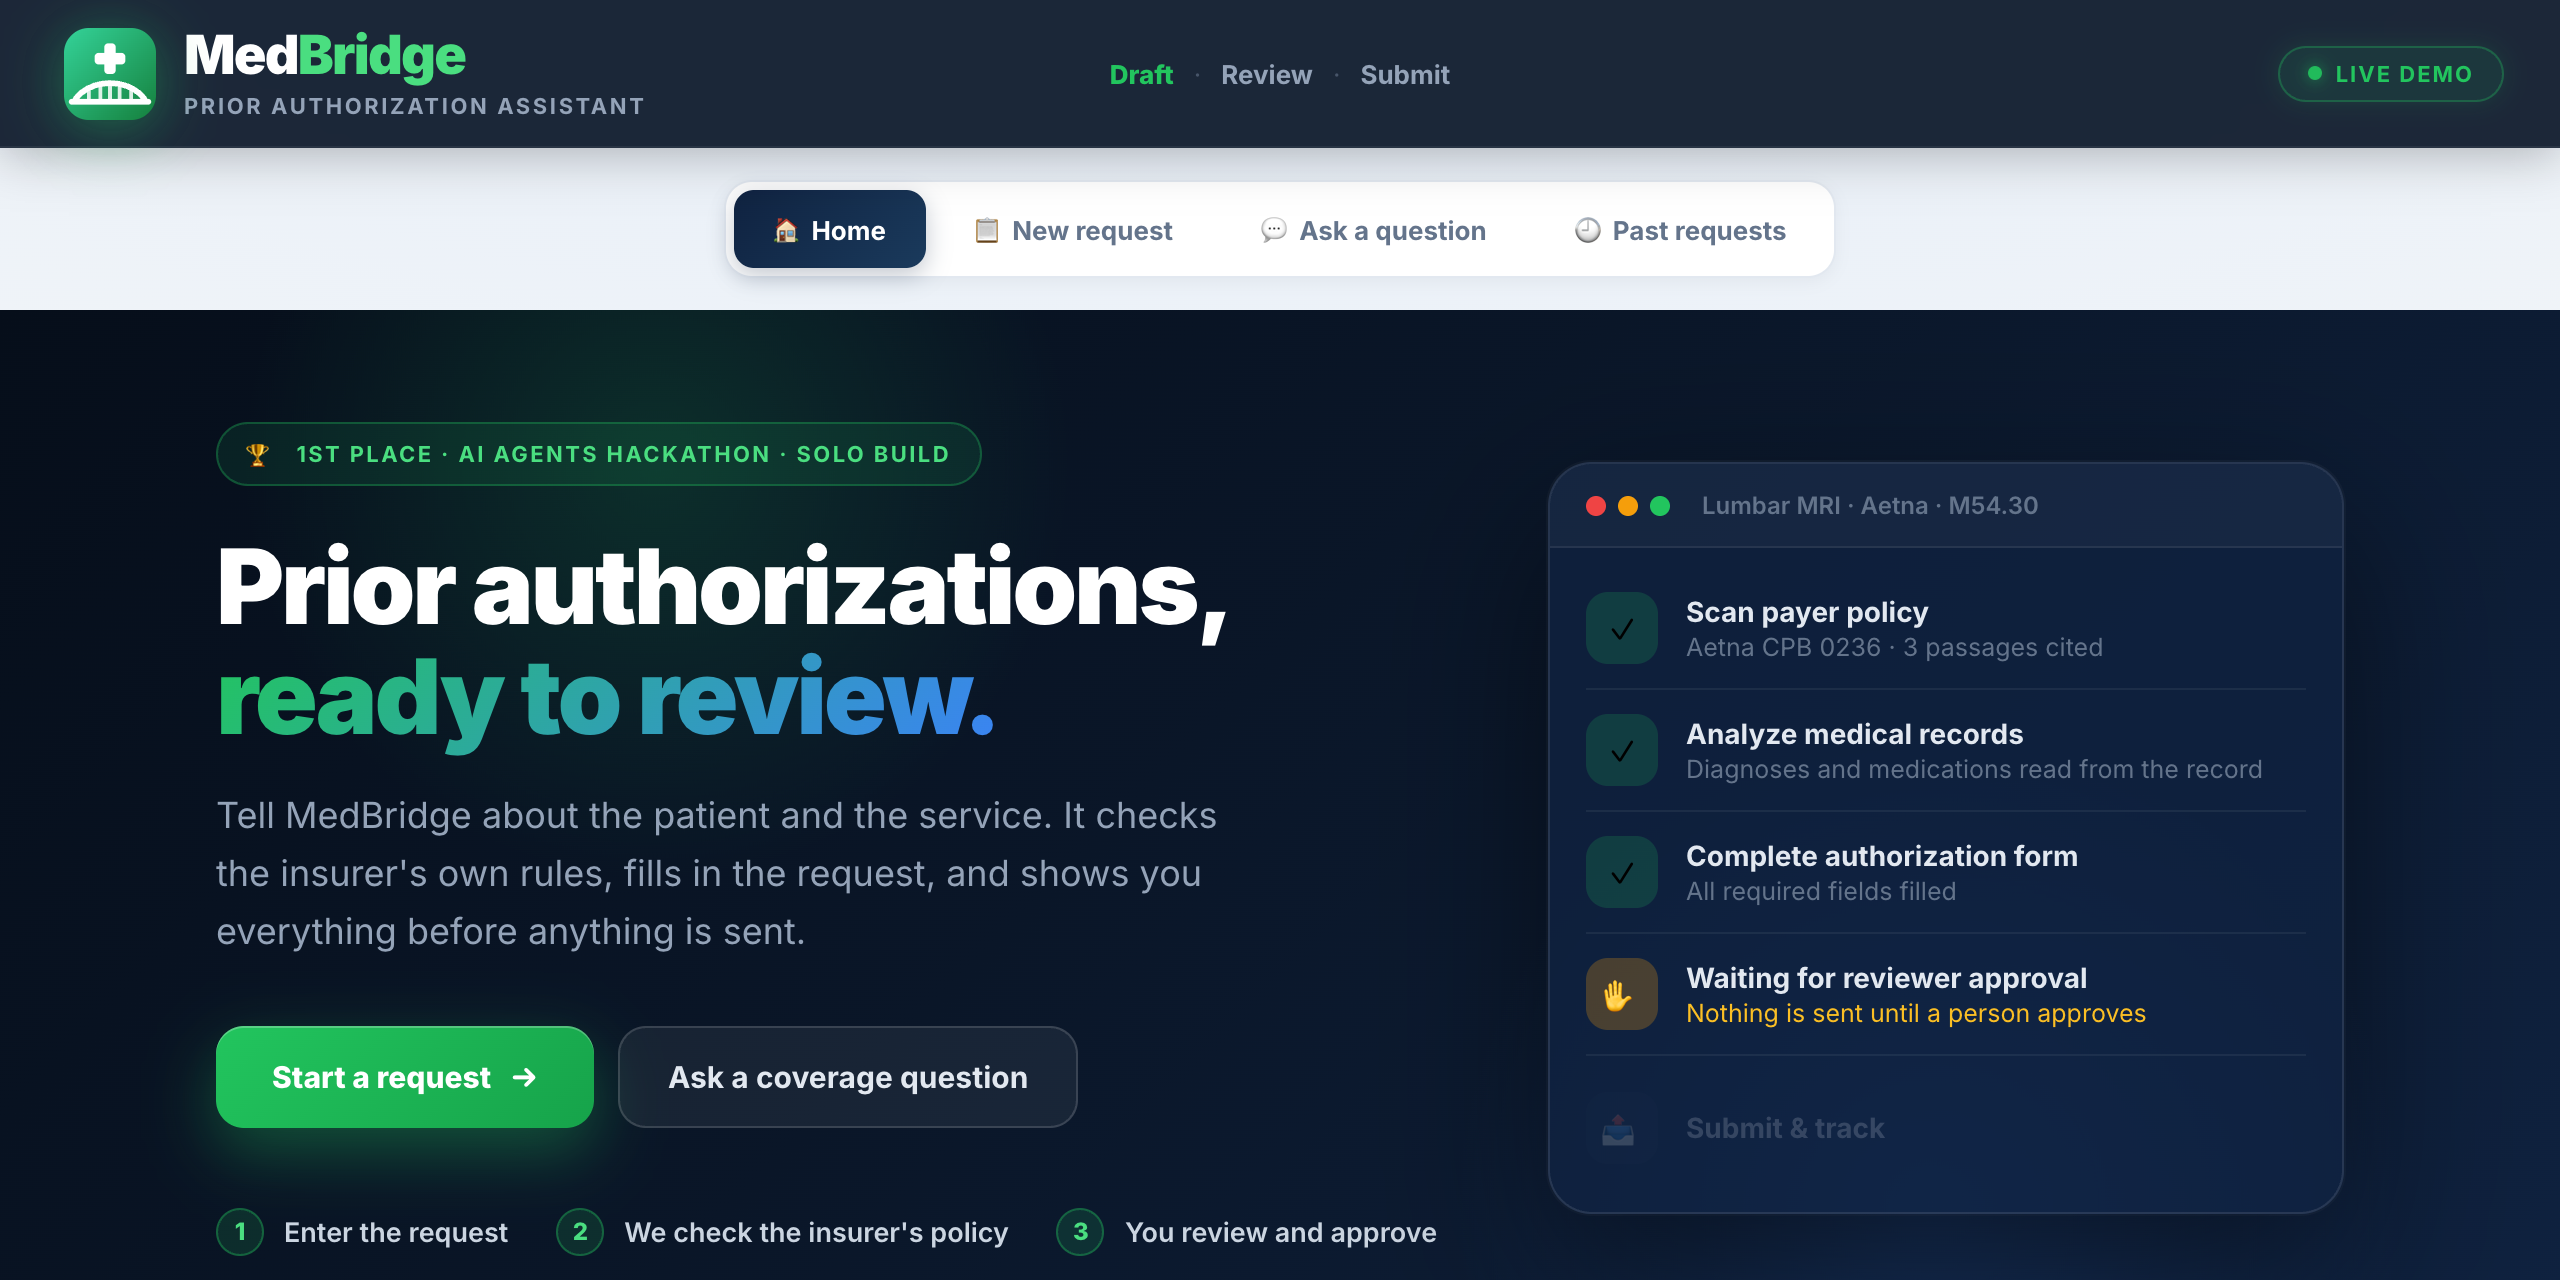
\includegraphics[width=\textwidth]{fig/cover_landing.png}
      \captionof{figure}{MedBridge prototype home screen. The animated card previews the agent's workflow: policy scan, record analysis, form completion, a pause for human approval, then submission and tracking. Screenshot of our own prototype. The project began as the \textbf{1st-place solo hackathon entry} described in Section~2.4.}
      \label{fig_teaser}
    \end{center}
}]

%%%%%%%%% BODY TEXT
\section{Abstract}
Prior authorization (PA) requires clinics to obtain insurer approval before many tests and treatments; the manual process delays care, and denials are rarely appealed although most appeals succeed. We extend \emph{MedBridge}, a \textbf{1st-place solo hackathon prototype}, into a policy-grounded assistant. From one structured request (patient, payer, service, diagnosis, justification), an LLM agent with retrieval over public payer and CMS policies prepares the form, pauses for human approval, submits, tracks the decision and, on denial, drafts a cited appeal; a companion chatbot answers coverage questions with sources. The output is an audited request or appeal draft. Clinics could save staff time and appeal more denials. Payer interfaces are simulated.

%-------------------------------------------------------------------------
\section{Introduction}

\subsection{Target Market}
Prior authorization is a documented burden. In an American Medical Association survey of 1{,}000 physicians (fielded December 2023, published June 2024), 94\% said it delays necessary care, 24\% reported a serious adverse event for a patient, and physicians reported completing an average of 43 requests a week, equal to about 12 hours of physician and staff time \cite{ama2024} (the AMA opposes prior authorization, so these are advocacy-group survey results). Denials are common and mostly reversed when challenged: in 2024 Medicare Advantage insurers fully or partially denied 4.1 million of 52.8 million requests, yet 80.7\% of appealed denials were overturned while only 11.5\% of denials were appealed \cite{kff2024}. Reported waits are contested: about two-thirds of physicians in an earlier AMA survey (2017 data) waited at least one business day and roughly 30\% three days or longer \cite{ama2018}, whereas insurer-reported median response times are about one day \cite{kffmetrics}. Manual handling is costly: in the 2019 CAQH Index a manual prior authorization cost providers \$10.92 against \$1.88 electronically \cite{caqh2019}. Federal rule CMS-0057-F additionally requires large payers (Medicare Advantage, Medicaid managed care and exchange plans) to offer prior-authorization APIs by January 2027 \cite{cms0057f}, so tooling that speaks structured requests is becoming relevant.

\subsection{Target Users}
The primary users are prior-authorization coordinators and administrative staff in outpatient clinics, who assemble requests from payer rules and chart notes. The secondary users are physicians, who review and sign appeals. Their needs are (i) knowing what a specific payer requires for a specific service, (ii) a correct, complete request the first time, (iii) a defensible appeal when a request is denied, and (iv) a record of who approved what.

\subsection{Why General LLMs Fall Short}
A general-purpose chatbot lacks current payer-specific criteria, cannot act on systems (prepare, submit, track, appeal), and gives untraceable answers, which is unacceptable when a wrong coverage claim ends up in a submission. MedBridge addresses these gaps with two techniques from the course: \textbf{Knowledge Augmentation \& Retrieval} (policy documents embedded in a vector database and retrieved per request) and \textbf{Agentic Workflows \& Tool Use} (a reasoning loop that chooses among tools and branches on denial).

%-------------------------------------------------------------------------
\subsection{Project Origin: Hackathon Winner, Then Extended}
\noindent\fbox{\parbox{\dimexpr\linewidth-2\fboxsep-2\fboxrule\relax}{\small
\textbf{MedBridge won 1st place at the AI Agents Hackathon, hosted by OSS4AI in collaboration with Beta Fund and Gravitational Ventures, and was built solo} \cite{medbridge_hackathon}. A hackathon judge's written feedback: ``Pre-approval is one of the most frustrating steps of treatment and solving it with an agentic AI approach is really novel.'' This paper describes how that prototype is rebuilt and extended for this course.}}

\smallskip
\noindent The hackathon version was a working agent: an LLM-driven loop over six tools (policy scan, record analysis, form fill, submission, status tracking, appeal drafting), a React interface that shows each step live, and simulated payer responses. Its policy data was hand-written, it submitted without a review step, and it had no evaluation. The extension for this course adds:
\begin{itemize}\itemsep0pt
\item retrieval over real public payer and CMS policy documents, replacing hand-written policy data;
\item a human approval gate and a persistent audit trail;
\item a cited policy chatbot;
\item a retrieval evaluation and a planned agent evaluation;
\item a provider-independent runner that adds Claude (Anthropic API) and Claude on Amazon Bedrock alongside Groq.
\end{itemize}

%-------------------------------------------------------------------------
\section{Related Work}
\textbf{Retrieval-augmented generation.} Lewis \etal\cite{lewis2020rag} combine a parametric generator with a non-parametric retriever to ground outputs in external text. Xiong \etal\cite{xiong2024medrag} benchmark RAG for medical question answering and report gains over prompting without retrieval. We apply the same principle to payer coverage policy, where documents differ by payer and change over time.

\textbf{Tool-using agents.} ReAct \cite{yao2023react} interleaves reasoning with actions and observations, and Toolformer \cite{schick2023toolformer} trains models to call APIs. MedBridge uses native function calling in a ReAct-style loop in which the model, not a fixed script, selects the next tool.

\textbf{Clinical language models.} Singhal \etal\cite{singhal2022medpalm} show that LLMs encode clinical knowledge but still need expert evaluation. We avoid relying on parametric medical knowledge and retrieve criteria at inference time.

\textbf{LLMs for prior authorization.} Pandey \etal\cite{pandey2024multiagent} split medical-necessity justification across specialized LLM agents and report high checklist accuracy with GPT-4. Vatsal \etal\cite{vatsal2024gpt} frame prior authorization as guideline-based question answering over patient records and report a mean weighted F1 of 0.61. Awan and Raza \cite{awan2026pa} find that LLM-drafted prior-authorization letters have strong clinical content but weak administrative elements such as missing billing codes. Selvaraj \etal\cite{selvaraj2026fairness} study the fairness of an automated prior-authorization system.

\textbf{Industry.} Vendors such as Cohere Health offer AI-assisted prior-authorization platforms to health plans \cite{cohere2025profile}, and patient-facing tools draft denial appeals \cite{pymnts2026appeals}; the success rates reported for these products are company claims.

\textbf{Gap.} The research works above evaluate judgments or letters in isolation, and the products serve payers or patients. To our knowledge, none combines retrieval over real payer policy documents, a tool-using agent, a human approval gate and denial-triggered appeal drafting with citations for clinic staff, which is the combination explored here.

%-------------------------------------------------------------------------
\section{Technical Contribution}
\textbf{Novelty.} The hackathon prototype supplied the agent loop and interface; the contributions below are new in this work. The contribution is an end-to-end, auditable pipeline rather than a new model: policy-grounded generation, agentic action, and enforced human review in one clinic-side workflow, with an evaluation protocol for each stage.
\begin{enumerate}
\item \textbf{Policy-grounded retrieval with payer scoping.} Public policy documents (Aetna Clinical Policy Bulletins, CMS National Coverage Determination 220.2, Blue Cross Blue Shield, UnitedHealthcare and Cigna policies) are chunked (160 words, 30-word overlap), embedded with all-MiniLM-L6-v2 \cite{reimers2019sbert} and stored in ChromaDB with source URL, payer and retrieval date. Queries are filtered to the requesting payer, and a payer with no documents returns nothing rather than another payer's policy.
\item \textbf{Human-in-the-loop gate inside the agent loop.} Outward-facing tools are marked as requiring approval. The loop blocks before such a tool runs until a reviewer approves or rejects, and every action is written to a persistent audit trail.
\item \textbf{Denial-conditioned appeal drafting with citation.} After a denial, the agent retrieves the policy passage that states the relevant criterion (for example, the conservative-therapy requirement) and quotes it in the draft appeal, which still requires physician review.
\item \textbf{Cited policy chatbot.} A conversational endpoint answers coverage questions only from retrieved passages, shows each source, and states when the collection does not cover a payer.
\item \textbf{Vertical-plugin architecture.} Tools, prompts and form schema live in one module per vertical; the agent runner, API and UI are generic. The runner supports Groq, Claude through the Anthropic API, and Claude on Amazon Bedrock, selected by one setting; the evaluations reported here ran on Groq, and Claude and Bedrock results are planned for Phase 2.
\end{enumerate}

%-------------------------------------------------------------------------
\begin{figure*}[t]
\centering
\resizebox{\textwidth}{!}{%
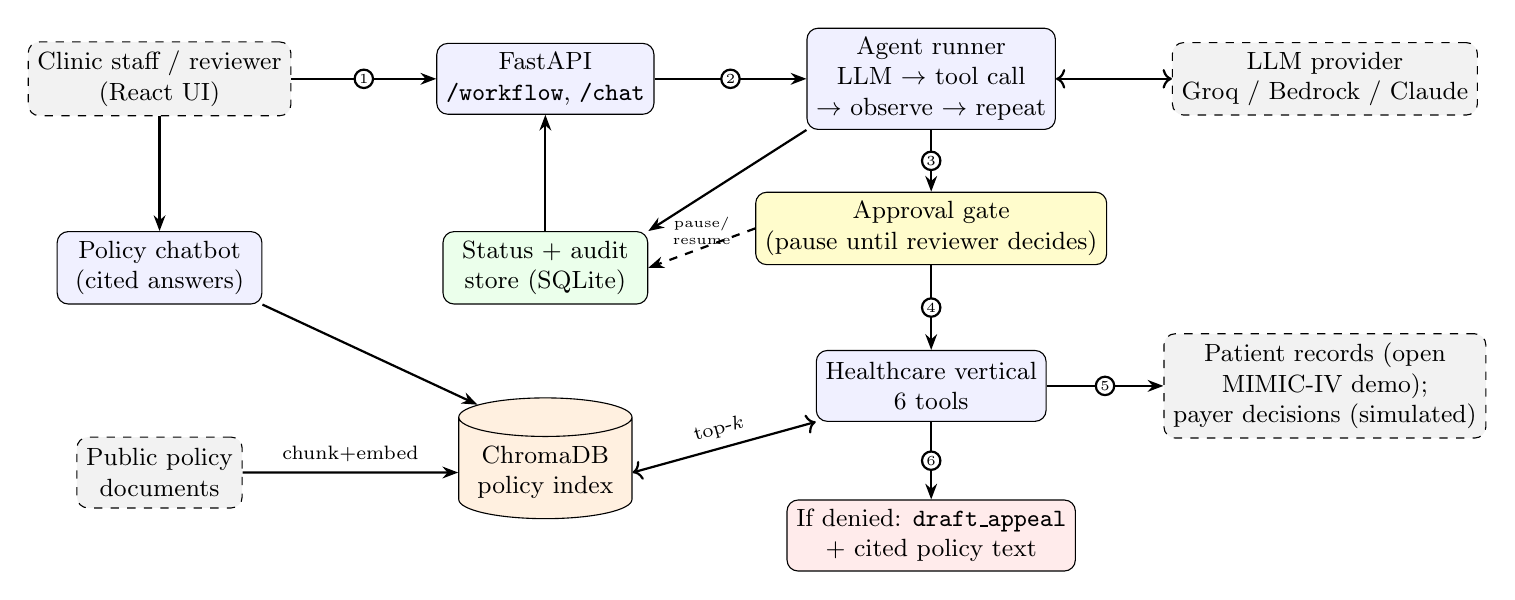
\begin{tikzpicture}[
  node distance=5mm and 9mm,
  box/.style={draw,rounded corners,align=center,minimum height=9mm,minimum width=26mm,font=\small,fill=blue!6},
  store/.style={draw,cylinder,shape border rotate=90,aspect=0.25,align=center,minimum height=11mm,minimum width=22mm,font=\small,fill=orange!12},
  ext/.style={draw,dashed,rounded corners,align=center,minimum height=9mm,font=\small,fill=gray!10},
  arr/.style={-{Stealth[length=2mm]},thick}]
\node[ext] (user) at (0,0) {Clinic staff / reviewer\\(React UI)};
\node[box] (api) at (4.9,0) {FastAPI\\\texttt{/workflow}, \texttt{/chat}};
\node[box] (loop) at (9.8,0) {Agent runner\\LLM $\to$ tool call\\$\to$ observe $\to$ repeat};
\node[ext] (llm) at (14.8,0) {LLM provider\\Groq / Bedrock / Claude};
\node[box,fill=yellow!20] (gate) at (9.8,-1.9) {Approval gate\\(pause until reviewer decides)};
\node[box,fill=green!8] (status) at (4.9,-2.4) {Status + audit\\store (SQLite)};
\node[box] (chat) at (0,-2.4) {Policy chatbot\\(cited answers)};
\node[box] (tools) at (9.8,-3.9) {Healthcare vertical\\6 tools};
\node[ext] (ehr) at (14.8,-3.9) {Patient records (open\\MIMIC-IV demo);\\payer decisions (simulated)};
\node[store] (vec) at (4.9,-5.0) {ChromaDB\\policy index};
\node[ext] (docs) at (0,-5.0) {Public policy\\documents};
\node[box,fill=red!8] (appeal) at (9.8,-5.8) {If denied: \texttt{draft\_appeal}\\+ cited policy text};
\draw[arr] (user) -- node[midway,circle,draw,fill=white,inner sep=0.7pt,font=\tiny]{1} (api);
\draw[arr] (api) -- node[midway,circle,draw,fill=white,inner sep=0.7pt,font=\tiny]{2} (loop);
\draw[arr,<->] (loop) -- (llm);
\draw[arr] (loop) -- node[midway,circle,draw,fill=white,inner sep=0.7pt,font=\tiny]{3} (gate);
\draw[arr] (gate) -- node[midway,circle,draw,fill=white,inner sep=0.7pt,font=\tiny]{4} (tools);
\draw[arr] (loop.south west) -- (status.north east);
\draw[arr,dashed] (gate.west) -- node[above,font=\tiny,align=center,inner sep=1pt]{pause/\\resume} (status.east);
\draw[arr] (status.north) -- (api.south);
\draw[arr] (user.south) -- (chat.north);
\draw[arr] (chat.south east) -- (vec.north west);
\draw[arr] (docs) -- node[above,font=\scriptsize]{chunk+embed} (vec);
\draw[arr,<->] (tools.south west) -- node[above,font=\scriptsize,sloped]{top-$k$} (vec.east);
\draw[arr] (tools) -- node[midway,circle,draw,fill=white,inner sep=0.7pt,font=\tiny]{5} (ehr);
\draw[arr] (tools) -- node[midway,circle,draw,fill=white,inner sep=0.7pt,font=\tiny]{6} (appeal);
\end{tikzpicture}}
\caption{Preliminary system design. Staff use the chatbot or submit a structured request. The agent loop calls tools, retrieving payer policy passages from the vector index; before the submission tool runs, the approval gate pauses the run until a reviewer decides. Status and the audit trail are persisted. A denial triggers a cited appeal draft. Numbers 1--5 trace the main request path and 6 is the denial branch. Dashed boxes are external to our code; patient records come from the open MIMIC-IV demo, while payer decisions and submission are simulated.}
\label{fig:system}
\end{figure*}

\section{Preliminary System Design}
Figure~\ref{fig:system} shows the components. A request flows: UI $\to$ FastAPI (background task) $\to$ agent runner. The runner sends the request and tool schemas to the LLM, executes whichever tool the model selects, appends the observation, and repeats until the model stops calling tools. The six tools cover policy retrieval (RAG), record analysis, form completion, submission, status tracking and appeal drafting. Before \texttt{submit\_authorization} runs, the gate sets the request to \emph{awaiting approval}; approval resumes the loop and rejection ends it. The chatbot shares the retriever but uses its own tool loop.

\textbf{Inputs and outputs.} Input: payer, member and patient identifiers, service, ICD-10 code and clinical justification, or a free-text policy question. Output: a completed and reviewed request with a step log and audit trail, a cited appeal draft on denial, or a cited answer.

\textbf{Technology stack.} The backend is FastAPI with SQLite for requests, steps and the audit trail, and ChromaDB with all-MiniLM-L6-v2 embeddings for retrieval. The agent runs on Groq, Claude through the Anthropic API, or Claude on Amazon Bedrock. The interface is React with Vite. Patient records come from the MIMIC-IV demo. Where the browser supports it, staff can dictate into the free-text request fields (patient name, physician name and clinical justification) with the browser's speech recognition; the transcript is appended to the field and the reviewer still checks it. Browser speech services process audio in the cloud, so dictation is only appropriate with demo data, and we have not evaluated its accuracy. An external dictation tool such as Wispr Flow can be used in the same way but is not integrated.

\textbf{Reviewer interface.} The approval screen is designed so that the reviewer sees the evidence before deciding. It shows a four-item checklist (policy evidence retrieved, patient record found, requested diagnosis on record, form completeness), each marked as on file, to be checked, or not available, and built only from signals the backend reports; the interface does not claim that a policy criterion is met or unmet, because the agent does not make that judgement. Each cited policy source opens the retrieved passage and a link to the full document, the same view is used for chatbot citations, and screens are labeled as simulated payer and demo data. Workflow steps appear on a timeline with their completion times. We have not yet run a usability study with clinic staff.

\textbf{Data.} The policy index is built from publicly available documents downloaded from their publishers (Aetna, CMS, Blue Cross Blue Shield of South Carolina, UnitedHealthcare, Cigna), with the retrieval date recorded per file. Patient records are read from the open MIMIC-IV Clinical Database Demo \cite{mimicdemo} (100 real, de-identified patients; Open Database License), loaded into SQLite; the agent looks a patient up by identifier and reports diagnoses, procedures and analgesic or NSAID medications on record. The demo contains hospital-admission data only, with no outpatient notes, so the record cannot confirm the duration of conservative therapy a payer requires, and the agent is told so. Payer decisions and submission are \emph{simulated}.

\textbf{Prototype status.} A working prototype implements the pipeline above. As a first check of retrieval, we labeled 29 questions with the document that answers each; with payer filtering, Recall@3 is 1.00 and MRR is 0.92, against Recall@3 of 0.86 and MRR of 0.70 without it. The questions were written by the author after reading the documents and the corpus is small (10 documents), so this is a sanity check, not a benchmark. The filter helps most where it removes plausible distractors: Aetna has five of the ten documents and 14 of the 29 questions, while every other payer has one or two documents, so for those payers the filter leaves very few candidates.

\textbf{Real denial cases.} On open data from the California Department of Managed Health Care \cite{dmhc_imr}, we selected the 64 independent medical reviews in which the request was an MRI of the lumbar spine; the reviewer overturned the health plan's denial in 33 of them (52\%). Using only each case's clinical description as the query (cut before any reasoning), retrieval returned a spine-MRI policy (Aetna CPB 0236 or BCBS CAM 709) at rank 1 for 94\% of cases and within the top 3 for 63 of 64, against about 20\%, 49\% and 67\% expected by chance at ranks 1, 3 and 5 (the chance that at least one chunk from the two spine-MRI policies appears among that many chunks drawn at random, since they make up about one fifth of the 171 indexed chunks). Relevance here is topic-level, not criterion-level, so this shows that retrieval finds the right policy, not that it finds the right criterion.

As a first agent check, with the approval gate auto-approved and a real MIMIC-IV demo patient, the expected six-tool sequence was produced in 5 of 5 runs for both the standard-approval and the denial-and-appeal scenario, with no tool errors; five runs is a small sample. A single run of the denial-and-appeal scenario on Claude Sonnet 4.6 through Amazon Bedrock also produced the expected sequence with no errors and cited Aetna CPB 0236; full Bedrock and Claude results are planned for Phase 2.

\textbf{Planned evaluation (Phase 2).} (1) Retrieval quality with chunk-size and filter ablations; (2) agent tool-sequence correctness over repeated runs on several LLM providers; (3) citation faithfulness of drafted appeals and chat answers, judged on a sample; (4) agent with RAG versus a static policy table.

\textbf{Limitations of the current design.} Simulated payer interfaces, patient data limited to the 100-patient open MIMIC-IV demo, no user authentication or roles, no HIPAA-grade handling of real patient data, a small policy corpus without Humana or Medicaid documents, and drafts that always require clinician review.

\section{Plan for Phase 2}
\begin{itemize}
    \item By Nov 10: run the agent and chatbot evaluations on Claude and on Amazon Bedrock as well as Groq; fix tool-order failures.
    \item By Nov 17: extend patient data (full MIMIC-IV if credentialing is approved, otherwise Synthea) and add a hand-labeled criterion-level evaluation.
    \item By Nov 24: extend the policy corpus; build the chatbot evaluation set.
    \item By Dec 1: ablations (retrieval settings, with versus without RAG).
    \item By Dec 8: complete methodology, results, discussion and limitations.
    \item Dec 15: final paper and code submission.
\end{itemize}

%-------------------------------------------------------------------------

{\small
\bibliographystyle{ieee_fullname}
\bibliography{refs_medbridge}
}

\end{document}
